\usepackage{shared/cs45}
\usepackage{tikz}
\usepackage{multicol}
\usepackage{xstring}
\usetikzlibrary{graphs}
\tikzset{>=latex}

\title{CS 45, Lecture 12}
\subtitle{Recent Unix Tools}
\date{Winter 2023}
\author{Akshay Srivatsan, Ayelet Drazen, Jonathan Kula}

\newcommand{\var}[1]{\texttt{\$#1}}
\newcommand{\sh}[1]{\mintinline{shell}{#1}}
\newcommand{\cmd}[1]{\texttt{#1}}

\newcommand{\magick}[4]{
  \begin{example}<only@+>[magick: #1]
    #2:

    \texttt{#3}
    \begin{center}
      \begin{tikzpicture}[node distance=0.5\textwidth]
        \node (before) {
          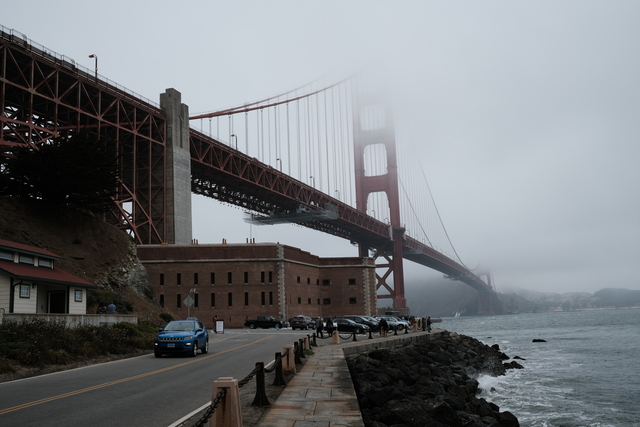
\includegraphics[scale=0.25]{images/magick/input.jpg}
        };
        \node (after) [right of=before] {
          \includegraphics[scale=0.25]{images/magick/#4}
        };

      \draw[->,thick] (before.east) -- (after.west);
      \end{tikzpicture}
    \end{center}
  \end{example}
}

\begin{document}

\maketitle

\frame{\titlepage}

\begin{frame}{Announcements}
  \begin{itemize}
    \item Assignment 5 is due today at 11:59 PM, contact us if you need an
      extension.
      \begin{itemize}
        \item Please either make a private post on Ed or email all three of us
          together, if you email just one of us we may miss it.
      \end{itemize}
    \item Assignment 6 will go out today or tomorrow.
    \item Final Project guidelines will go out soon (and we'll talk about it in
      a second).
  \end{itemize}
\end{frame}

\begin{frame}{Final Projects}
  Task:
  \begin{itemize}
    \item Pick a tool or concept related to this class (either one we've
      covered or one we didn't cover but you're interested in).
    \item Do research on what it's for/how it works/how you use it.
    \item Write a short guide on how/when to use the tool.
    \item Make a few slides describing the tool and giving example use cases.
  \end{itemize}
  Logistics:
  \begin{itemize}
    \item Due on March 20, 2023 (Monday of Finals Week).
  \end{itemize}
\end{frame}

\begin{frame}
  \frametitle{Outline}
  \tableofcontents[hidesubsections]
\end{frame}

\section{Overview}

\begin{frame}{What's wrong with the old tools?}
  For the most part, they're okay, but\textellipsis
  \pause
  \begin{itemize}
    \item They only work on text files.
      \pause
    \item They're (mostly) single-threaded.
      \pause
    \item They don't take advantage of new discoveries and inventions.
      \pause
    \item Their interface is so standardized that they can't innovate.
  \end{itemize}
\end{frame}

\begin{frame}{Types of Tools}
  \begin{description}
    \item[upgrades:] modernized versions of the traditional tools you know
      \pause
    \item[swiss army knives:] bundles of many related tools
      \pause
      \begin{itemize}
        \item Kind of like Git; Git contains \texttt{add}, \texttt{commit},
          \texttt{merge}, etc.
      \end{itemize}
    \pause
  \end{description}

  \vfill

  The point of this lecture is \textbf{not} that you become an expert in these
  tools!
  \pause

  We're showing you these tools so you know that they exist, because we think
  they're useful (and/or really cool).
\end{frame}

\section{Upgrades}

\begin{frame}[fragile]{ripgrep}
  \begin{itemize}
    \item \href{https://github.com/BurntSushi/ripgrep}{Ripgrep} is an upgraded
      version of \cmd{grep} and \cmd{find}
    \item Its main selling points are that it's fast and it's
      \enquote{ergonomic}.
  \end{itemize}
  \pause
  \vfill
  \begin{example}<only@+>[ripgrep for text]
    Searching for a file in the current directory (or subdirectories) containing the text \enquote{hello}:
    \begin{minted}{shell}
      rg hello
    \end{minted}
  \end{example}
  \begin{example}<only@+>[ripgrep for regex]
    Searching for a file in the current directory (or subdirectories) containing the regular expression \texttt{/hello.*!/}:\mode<article>{\footnote{Surrounding a regular expression with slashes (like you do when using \texttt{sed} is a common way of distinguishing it from an ordinary string. Some languages (like JavaScript) even support it as part of their syntax!}}
    \begin{minted}{shell}
      rg 'hello.*!'
    \end{minted}
  \end{example}
  \begin{example}<only@+>[ripgrep in a file]
    Searching for lines of \cmd{student\_hobbies.txt} containing the string \cmd{akshay01}:
    \begin{minted}{shell}
      rg akshay01 student_hobbies.txt
    \end{minted}
  \end{example}
\end{frame}

\begin{frame}[fragile]{fd}
  \begin{itemize}
    \item \href{https://github.com/sharkdp/fd}{fd} is a user-friendly
      alternative to \cmd{find}
    \item Its main selling point is that it's much more intuitive than \cmd{find}
  \end{itemize}
  \pause
  \vfill
  \begin{example}<only@+>[fd for files named \enquote{grep}]
    Search the current directory and all subdirectories for every file with
    \enquote{grep} in its name:
    \begin{minted}{shell}
      fd grep
    \end{minted}
  \end{example}
  \begin{example}<only@+>[fd for symbolic links]
    Search for every symbolic link in the current directory or its subdirectories:
    \begin{minted}{shell}
      fd --type symlink
    \end{minted}
  \end{example}
  \begin{example}<only@+>[fd all large files]
    Search for every file greater than or equal to 500 MB in size and print out
    a helpful message:
    \begin{minted}{shell}
      fd --size +500MB --exec echo You should delete {/} in directory {//}
    \end{minted}
  \end{example}
\end{frame}

\begin{frame}[fragile]{exa}
  \begin{itemize}
    \item \href{https://github.com/ogham/exa}{exa} is a modern alternative to
      \cmd{ls}
    \item Its main selling point is that it has more features than \cmd{ls},
      like viewing your current git status (and it's colorful!)
  \end{itemize}
  \pause
  \vfill
  \begin{example}<only@+>[exa: sort files by size]
    List all the files in the current directory, ordered by size
    \begin{minted}{shell}
      exa --sort=size
    \end{minted}
  \end{example}
  \begin{example}<only@+>[exa: git status]
    List every file in the current directory's git status:
    \begin{minted}{shell}
      exa --long --git
    \end{minted}
  \end{example}
  \begin{example}<only@+>[exa: tree]
    Show a tree of files in the current directory and all subdirectories:
    \begin{minted}{shell}
      exa --tree
    \end{minted}
  \end{example}
\end{frame}

\begin{frame}[fragile]{fish}
  \begin{itemize}
    \item \href{https://fishshell.com/}{fish} is a modern alternative to
      \cmd{bash} and \cmd{zsh}.
    \item Its main selling points are that it has a lot more conveniences, like autosuggestions and a nicer scripting language.
      \pause
    \item It is \textbf{not} backwards compatible with \cmd{sh}!
  \end{itemize}
  \pause
  \vfill
  \begin{center}
    [Demo Time]
  \end{center}
\end{frame}

\section{Swiss Army Knives}

\subsection{Images}
\begin{frame}{Images}
  \begin{itemize}
    \item Images exist.\textsuperscript{[citation needed]}
    \pause
    \item Sometimes, we want to modify those images.
    \pause
    \item Images are, notably, \textbf{not} text files, so our usual Unix
      commands won't work.
    \pause
    \item \textit{ImageMagick} is a set of tools for working with images.
  \end{itemize}
\end{frame}

\begin{frame}[fragile]{ImageMagick}
  ImageMagick is broken into subcommands:
  \begin{description}
    \item[convert] is the one you usually want (and the default), it modifies a file
    \item[mogrify] modifies a file in-place (overwriting the original)
    \item[display] opens an image in a window
    \item[compare] diffs two images
  \end{description}
\end{frame}

\begin{frame}[c,fragile]{ImageMagick Convert}
  \magick{png to jpg}{Convert a \texttt{jpg} file to a \texttt{png} file}{
    magick convert input.jpg output.png
  }{output.png}
  \magick{compress}{Compress an image}{
    magick convert input.jpg -quality 50 output.jpg
  }{compressed.jpg}
  \magick{resize}{Resize an image}{
    magick convert input.jpg -resize 320x240 output.jpg
  }{resized.jpg}
  \magick{grayscale}{Make an image grayscale}{
    magick convert input.jpg -colorspace gray output.jpg
  }{gray.jpg}
  \magick{brightness}{Brighten an image}{
    magick convert input.jpg -modulate 200,100,100 output.jpg
  }{bright.jpg}
  \magick{saturation}{Saturate an image}{
    magick convert input.jpg -modulate 100,200,100 output.jpg
  }{saturated.jpg}
  \magick{hue}{Hue an image}{
    magick convert input.jpg -modulate 100,100,150 output.jpg
  }{hued.jpg}
  \magick{rotate}{Rotate an image}{
    magick convert input.jpg -rotate 180 output.jpg
  }{rotated.jpg}
  \magick{negate}{Get a negative image}{
    magick convert input.jpg -negate output.jpg
  }{negative.jpg}
  \magick{crop}{Crop an image}{
    magick convert input.jpg -crop 320x240+0+0 output.jpg
  }{cropped.jpg}
  \magick{caption}{Caption an image}{
    magick convert input.jpg -pointsize 56 -gravity south -fill white -annotate +0+0 "Karl the Fog" output.jpg
  }{captioned.jpg}
  \only<+> {
      There's a bunch of other things ImageMagick can do!  Their website has
      a full list.
  }
\end{frame}

\subsection{Documents}
\begin{frame}{Documents}
  \begin{itemize}
    \item Sometimes we need to work with formatted documents.
    \pause
    \item We \textit{could} use Google Docs or MS Word, but what if we need
      to work with a \text{lot} of documents?
    \pause
    \item There's a million incompatible document formats (Text, RTF, Word,
      ODT, PDF, HTML, Markdown, AsciiDoc, \LaTeX, EPUB, DocBook, etc.), and trying to find the right tool for each one is hard.
    \pause
    \item \textit{Pandoc} is \enquote{a universal document converter} that
      can work with all these formats!
  \end{itemize}
\end{frame}

\begin{frame}[fragile]{Pandoc}
  Pandoc is really just for converting between formats:
  \vfill
  \begin{example}<only@+>[pandoc]
    Converting between formats:
    \begin{minted}{shell}
    pandoc input.md -o output.docx
    \end{minted}
  \end{example}
  \begin{example}<only@+>[pandoc: multiple files]
    Combining files and converting between formats:
    \begin{minted}{shell}
    pandoc title.md body.md epilogue.md -o output.docx
    \end{minted}
  \end{example}
  \begin{example}<only@+>[pandoc: HTML fragment]
    Converting a Word Doc into an HTML fragment:
    \begin{minted}{shell}
    pandoc input.docx -o fragment.html
    \end{minted}
  \end{example}
  \begin{example}<only@+>[pandoc: HTML page]
    Converting a Word Doc into an HTML website (e.g., a blog post):
    \begin{minted}{shell}
    pandoc input.docx --standalone --metadata title="My Website" -o
    fragment.html
    \end{minted}
  \end{example}
  \begin{example}<only@+>[pandoc: PowerPoint]
    Converting a Markdown file into a slideshow:
    \begin{minted}{shell}
    pandoc input.md -o output.pptx
    \end{minted}
    \begin{center}
      [Demo Time (Again)]
    \end{center}
  \end{example}
  \begin{example}<only@+>[pandoc: PDF Slides]
    Converting a Markdown file into a PDF slideshow:
    \begin{minted}{shell}
    pandoc input.md -to beamer -o output.pdf
    \end{minted}
  \end{example}
  \vfill
  Once you've converted a file with Pandoc, you can edit it using
  whatever program you'd normally use.
\end{frame}

\subsection{Videos}
\begin{frame}{FFmpeg}
  \begin{itemize}
    \item Dealing with videos is a pain.
    \pause
    \item There are video container formats: Matroksa, MPEG-4, QuickTime, Audio Video Interleave, WebM, Ogg
    \pause
    \item There are video encoding formats: HEVC, H.264, AV1, VP9, VP8
    \pause
    \item There are audio encoding formats: AAC, MP3, Opus, FLAC
    \pause
    \item There are audio/video settings: bitrate, fps, resolution, sample
      rate
    \pause
    \item \textit{FFmpeg} is a tool to record, convert, and stream
      audio/video.
    \pause
    \item \textit{FFmpeg} also has a million different options and
      settings\textellipsis{} ask a search engine if you ever need to use it.
  \end{itemize}
\end{frame}

\begin{frame}[fragile]{FFmpeg Examples}
  FFmpeg examples from my command history:
  \vfill

  \begin{example}<only@+>[ffmpeg: record]
    Recording a video (on Linux):

    \texttt{ffmpeg -f v4l2 -framerate 30 -video\_size 1280x720 -i /dev/video4 recording.mkv}
  \end{example}
  \begin{example}<only@+>[ffmpeg: container]
    Change a video container:

    \texttt{ffmpeg -i input.webm -vcodec copy -acodec copy screen.mkv}
  \end{example}
  \begin{example}<only@+>[ffmpeg: encoding]
    Reëncoding a video:

    \texttt{ffmpeg -i input.webm -vcodec h264 -acodec copy screen.mkv}
  \end{example}
  \vfill
\end{frame}

\begin{frame}{Miscellanea}
  \begin{itemize}
    \item If you choose to research a tool for your final project, your slides
      might look like today's:
    \begin{itemize}
      \item What problem does this tool solve?
      \item What does the tool do?
      \item How do you use the tool?
    \end{itemize}
    \pause
    \item If you have fewer than six points by now (according to the guide from
      Lecture 1), come talk to us.
  \end{itemize}
\end{frame}

\end{document}
